\chapter{MODELING}
\label{chapter:modeling}

\par
The modeling phase included getting familiar with concepts of \acrshort{bsc}, creating the behavioral models for most of its functional parts, verifying its correctness and  defining the layered structure or models.

\section{Brainloop Secure Client app for iOS platform} 

\par
In order to deeply understand the concept behind \acrshort{bsc} we need to first have a good understanding of the Brainloop Secure Dataroom Service (\acrshort{bdrs}). 

\par
\acrshort{bdrs} \cite{BDRS_Description} is a secure service for data governance, allowing customer businesses a reliable and secure data and communication management  within the company as well as with the outside parties. To ensure a high level of security \acrshort{bdrs} makes use of different security mechanisms like two way authentication using time-limited PINs and 256-bit encryption of both storage and data transfer. Additionally application and system administration are separated, making them more secure.
The software also offers document management, which includes standard features like editing and filing of documents, but also has some more advanced features like document collections which combine multiple documents and allow easy sorting and structuring for them, while providing separate version control and different access rights for each document.

\par
\acrshort{bsc}'s \cite{BSC_UserGuide} is used to be able to conveniently access the secure datarooms in the \acrshort{bdrs} from iOS devices such as iPhone and iPad. The key features available to users are accessing the documents, boardbooks, votes and the events. The users can also download documents locally, annotate the protected PDF documents, share its reviews with other members of dataroom and sending the documents to internal as well as external email addresses according to the dataroom's security policy.

\par
The typical usage of the \acrshort{bsc} would be as follows: a user defines an access code, they get logged in with the correct credentials to the \acrshort{bdrs}, then they can choose which datarooms should be syncronized locally from the list of datarooms to which they were invited to. After these steps the user is eligible to use all the functionalities described above. If the application gets locked, the user needs to unlock it by typing the access code which was defined in the first step.

\section{Model description for Graphwalker}
\par
Like other \acrshort{fsm}s that are applied to \acrshort{mbt}, in the Graphwalker the \acrshort{fsm} and \acrshort{efsm} are represented in the form of a directed graph in which the vertexes represent states of \acrshort{aut} and the edges represent the transitions between the states. \acrshort{fsm}s can be created in a .graphml format with a yEd Graph Editor.

\par
The Graphwalker doesn't consider the styles and colors of vertexes and edges, as in order to differentiate between the edges and the vertexes in the provided report often \texttt{e\_} and \texttt{v\_} prefixes are used respectively. However using the prefixes is not mandatory.

\par
Graphwalker provides a way to initialize the variables within the vertex labels with \texttt{INIT} keyword, e.g. \texttt{INIT:condition = true;}. it can be either a local or a global variable, which means that it can be either used only in the model (local) where it is initialized, or it can be used in all the other models (global). These variables are then used in guards and actions. A guard defines the condition for Graphwalker to traverse the edge. e.g. \texttt{[condition == true]} guard would mean that this edge can be taken by the Graphwalker while traversing only if the condition is true. Only the edges can be annotated with guards. Similarly, the actions can be applied only to the edges. The actions are used to set the value of the variables in model. \texttt{/condition = false;} action would tell the Graphwalker to set the variable with name condition to false whenever the edge annotated with this action is taken in to traversal. If the  variable named condition is used for the first time in an action, that will also initialize the variable. 

\par
There are multiple keywords supported by the Graphwalker such as, \texttt{Start}, \texttt{SHARED}, \texttt{BLOCKED}, \texttt{INIT}, \texttt{REQTAG} and \texttt{weight}. The Start keyword stands for the starting vertex. It is not mandatory to have it in the model, however it needs to be specified to the Graphwalker, as a parameter given during the runtime to define the state it should start the traversal from. When multiple models are traversed together, the \texttt{SHARED} keyword would mean that the Graphwalker encountering a vertex in this model can be found in other models as well and for the next step the Graphwalker will consider all the edges coming out from current state in all the models. The \texttt{REQTAG} keyword can only be used for vertexes and usually gives information about the external requirements. Users can give specific weights to the edges in a model with the weight keyword. Ideally the weight should be between 0.0 and 1.0. During a random exploration of the model the value of weight would provide the Graphwalker with the probability that should be chosen to annotate the edge.

\section{Modeling of Brainloop Secure Client}

\par
Modeling of the \acrshort{bsc} behaviour included  most of its functionality for which separate models, interconnected using shared steps, where created. Some of the functional parts such as remote synchronization, boardbooks, offline usage, locking of the application, locking of the device and other environmental constraints were omitted during the modeling process, due to the time and complexity constraints.

\par
The model by its definition should be an abstracted representation of the system's behaviour.
The case-study from Silva et. al. \cite{Silva_SpecExplorer} showed that if the model is concretized down to the atomic actions of a user such as clicking a button and typing text, modeling requires huge effort which results in 40\% of lines of code of system implementation. But, according to Pretschner et. al. \cite{Pretschner_MBTInPractice} defining an adequate level of abstraction continues to be an art. So there is no premade recipe for that. In our models, we abstracted the transitions to the level where one transition contains the complete set of actions needed to bring the application to the last expected result in that test case. More detailed representation of abstracted transitions and states can be observed in attached figures in subsequent subsections.

\subsection{Modeling of Authentication}
\par
The authentication functionality of the \acrshort{bsc} consists of 2 steps. Defining the access code for accessing the application and the authentication against \acrshort{bdrs}. The access codes can be defined either as simple or complex. The difference between the two is that a simple access code can only contain numeric characters while the complex one can consist of alphanumeric characters and symbols. The defined access code is required to confirm the identity every time the application is run and also to unlock the application using its automatic lock feature, which occurs due the application idle time defined in the settings.

\par
Four different models were created for the authentication feature of the \acrshort{bsc}, which are Define Simple Access Code (with 7 state and 10 transitions), Define Complex Access Code (with 5 state and 7 transitions), Enter Access Code (with 8 state and 11 transitions) and Initial Authentication Against \acrshort{bdrs} (with 6 state and 9 transitions). The Define Simple Access Code model can be observed in the figure \ref{Fig:Authentication_Model_Screenshot}.

\begin{figure} [htbp!]
	\centering
					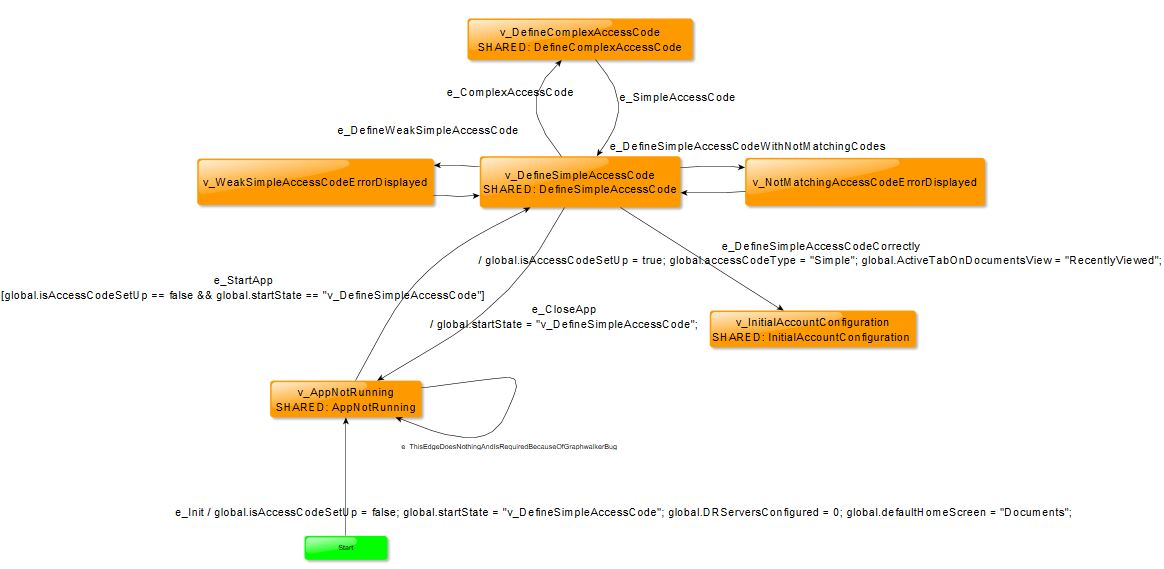
\includegraphics[width=1\textwidth]{figures/Authentication_model_screenshot}
					\caption{\label{Fig:Authentication_Model_Screenshot} Model for Define Simple Access Code feature}
\end{figure}

\subsection{Modeling of the Navigation between the tabs}
\par
After finishing the authentication steps in \acrshort{bsc}, the user is introduced to the internal application functionality which consists of the following five tabs: The documents tab, events tab, votes tab, datarooms tab and settings tab. A single model is devoted for describing only the navigation opportunities between these tabs. It contains all the possible transitions from one tab to another which also includes the closing of the application from any tab. The user can disable the votes and events tabs through the settings, for which the navigation model contains variables that are set in the settings tab for enabling and disabling the tabs. These variables are used in the guards of the navigation model. The model consists of 6 states and 25 transitions. The same is depicted in the figure \ref{Fig:Navigation_Model_Screenshot}.

\begin{figure} [htbp!]
	\centering
					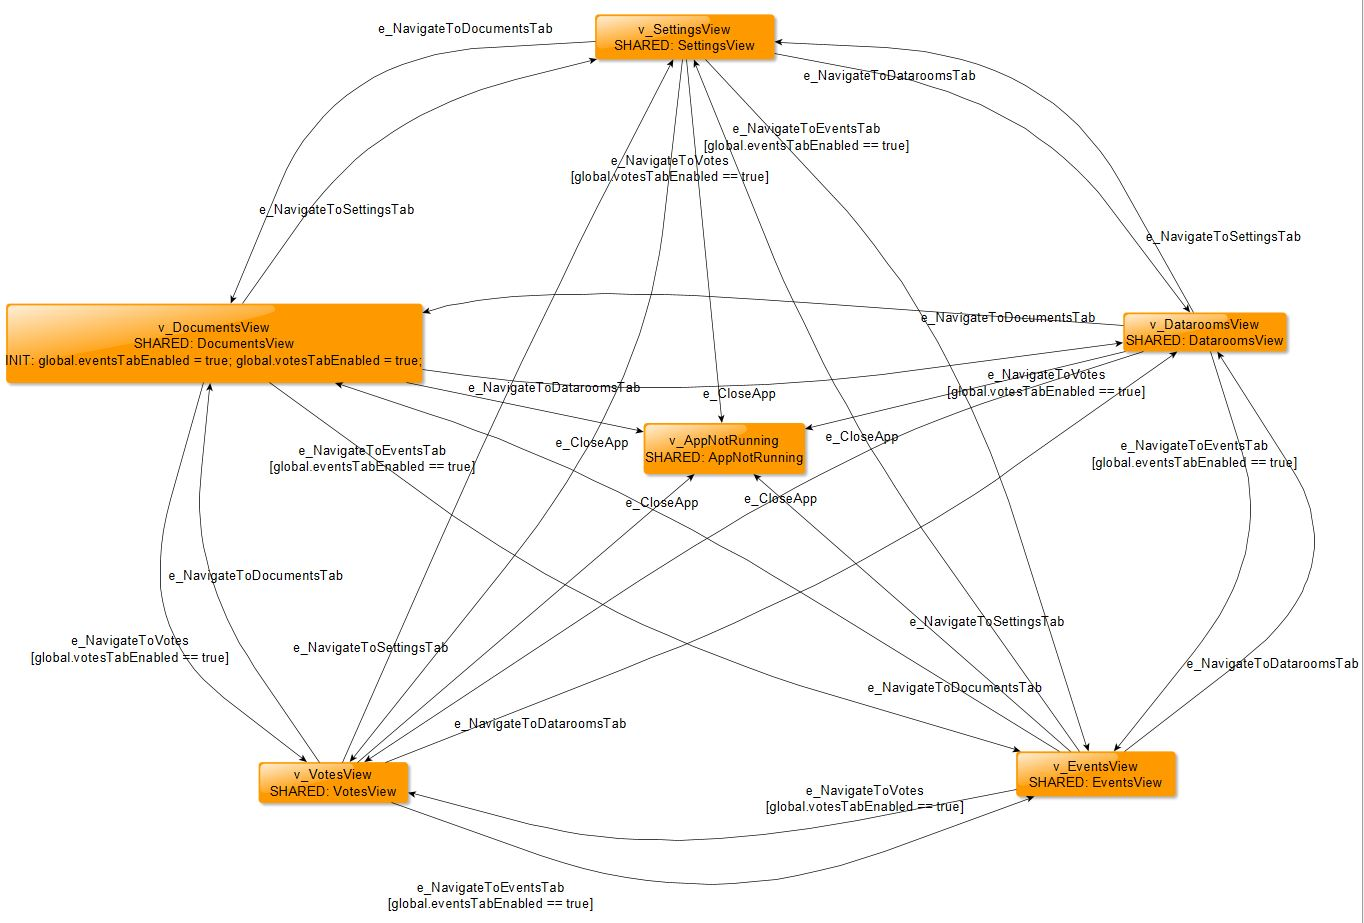
\includegraphics[width=0.92\textwidth]{figures/Navigation_model_screenshot}
					\caption{\label{Fig:Navigation_Model_Screenshot} Model for Navigation through Tabs}
\end{figure}

\subsection{Modeling of the Documents Tab}
\par
The documents tab is the most used tab in the \acrshort{bsc} as it provides a convenient representation of the documents residing in the datarooms. It is has four different options for filtering the documents, out of which two options are available by default. The recently viewed filter option shows the documents that were opened by the user during the usage of the \acrshort{bsc}, sorted based on the access time in descending order. The recently changed filter option displays documents that were recently added or modified within the synchronized datarooms, sorted based on the update date in descending order.

\par
The functionality of the documents tab is divided into three different models. The documents model is responsible for the navigation between the filter options, while the recently changed and recently viewed models describe the functionality provided to the user through the use of these filter options. The functionality could be accessing files or different types of file content, context menus as well as navigating back to the respective filter option. The recently viewed and recently changed models contain 7 states and 10 transitions each while the documents model has 5 states and 20 transitions. The documents model can be observed in the figure \ref{Fig:Documents_Model_Screenshot}. 

\begin{figure} [htbp!]
	\centering
					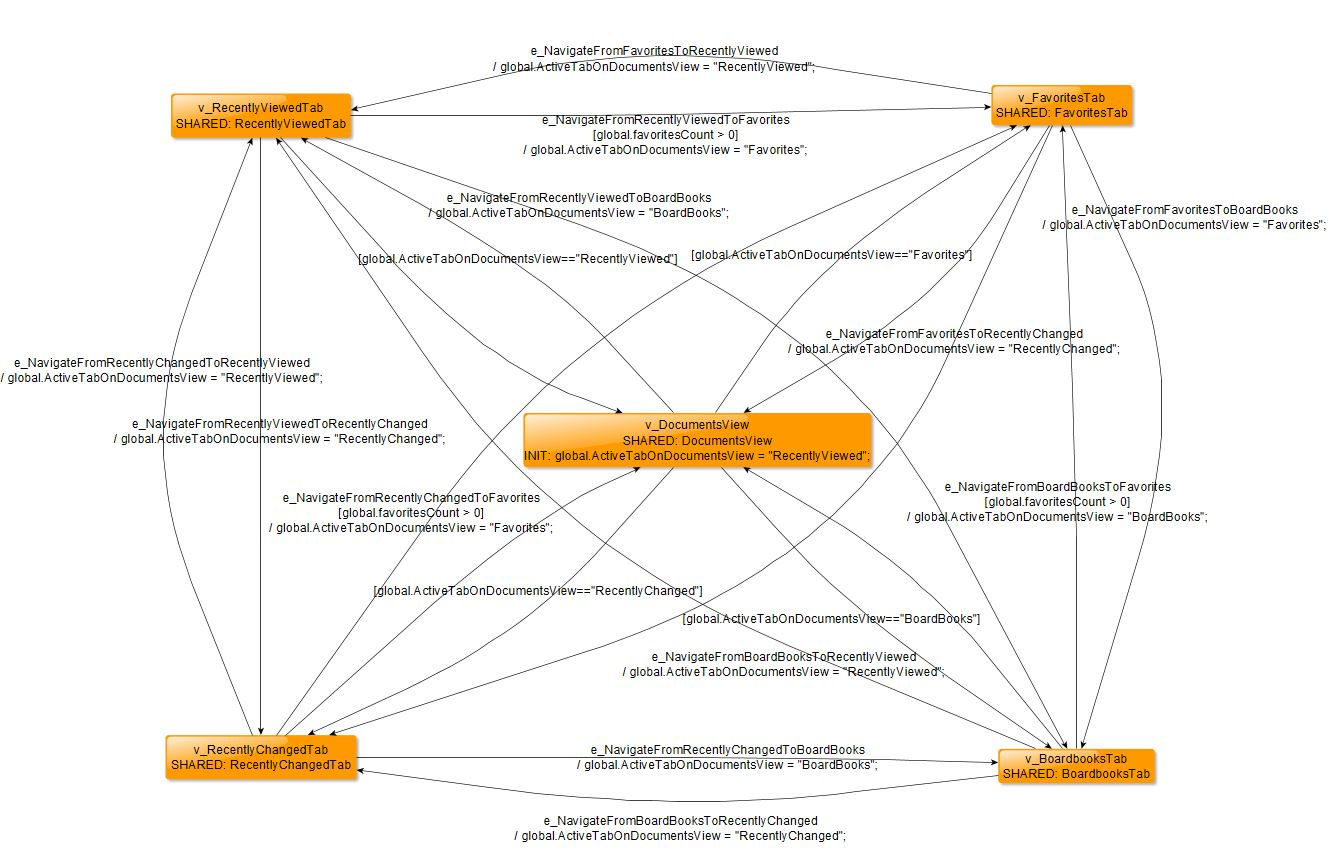
\includegraphics[width=0.92\textwidth]{figures/Documents_model_screenshot}
					\caption{\label{Fig:Documents_Model_Screenshot} Model for Documents Tab}
\end{figure}


\subsection{Modeling of the Events Tab}
\par
The organizational events is one of the features of the \acrshort{bdrs} which allows the user to access the created events of the synchronized datarooms in the \acrshort{bsc} through the events tab. There are multiple filtering options available which are, all events, past events, declined events, upcoming events and events for which the user's reply is pending. The displayed events can be sorted either based on the name or the due date. The user has the following three options to respond to an event which are accepting, declining or a tentative response, and this response is further synchronized with the \acrshort{bdrs}. The user can observe other participants of the event as well as the attachments that are available. The behavioral model of the events tab consists of 16 states and 30 transitions and can be observed in the figure \ref{Fig:Events_Model_Screenshot}.

\begin{figure} [htbp!]
	\centering
					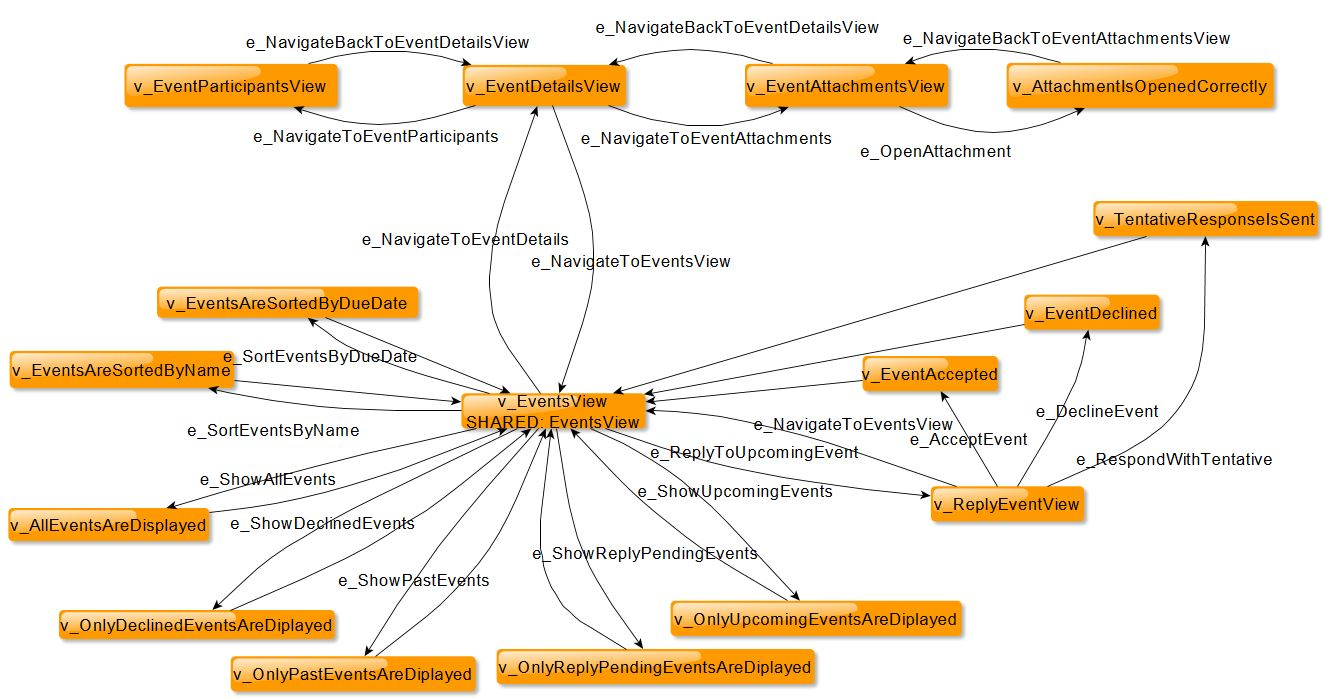
\includegraphics[width=1\textwidth]{figures/Events_model_screenshot}
					\caption{\label{Fig:Events_Model_Screenshot} Model for Events Tab}
\end{figure}

\subsection{Modeling of Votes Tab}
\par
The \acrshort{bdrs} supports a functionality called voting. In this function the user has the ability to access votes of the synchronized datarooms in the \acrshort{bsc} through the votes tab. The votes are filtered based on the following criteria which are, all votes, votes in progress, closed votes and votes for which the user's choice is pending. Similar to the events, the votes can be also sorted either based on the name or the due date. The above mentioned types of votes can be cast as either approved, declined or abstained. The user can observe the list of voters and attachments to these votes when expanding a specific vote. The behavioral model of the votes tab has 15 states and 30 transitions and can be observed in the figure \ref{Fig:Votes_Model_Screenshot}.

\begin{figure} [htbp!]
	\centering
					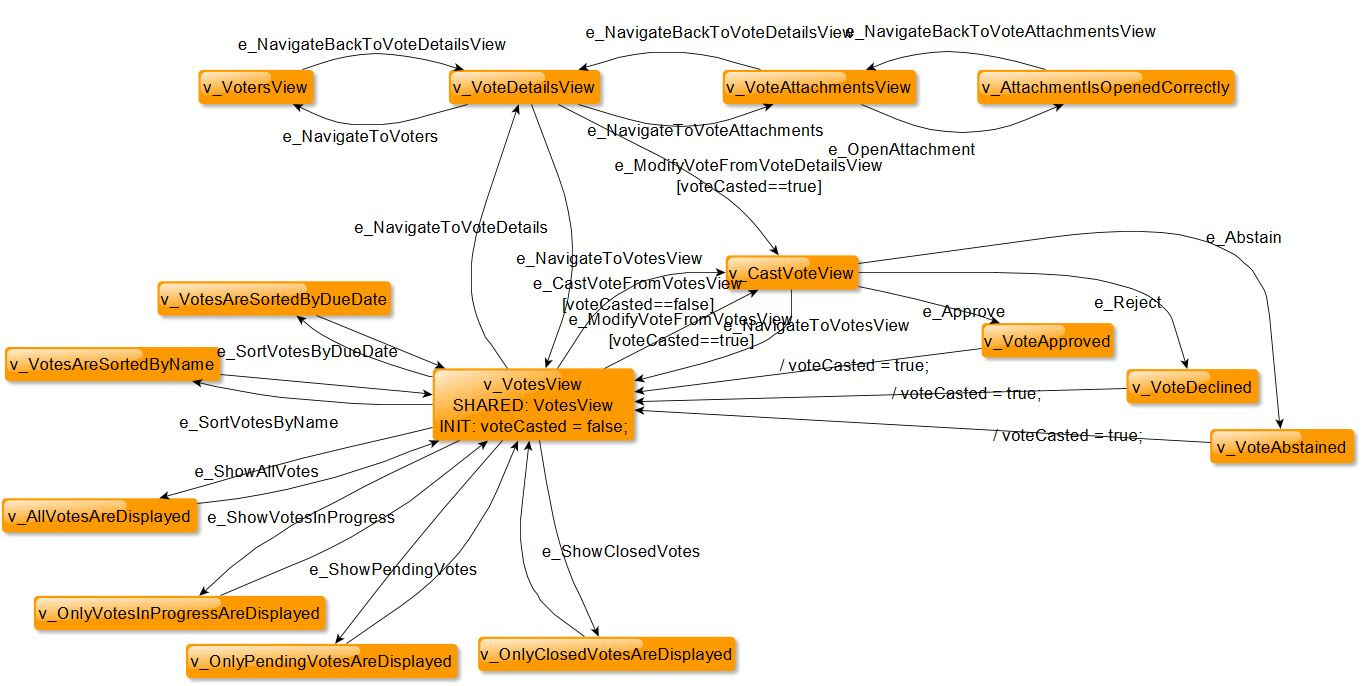
\includegraphics[width=1\textwidth]{figures/Votes_model_screenshot}
					\caption{\label{Fig:Votes_Model_Screenshot} Model for Votes Tab}
\end{figure}

\subsection{Modeling of the Datarooms Tab}
\par
The datarooms tab is the part of the \acrshort{bsc} where most of the application's functionality is embedded. The user can access all datarooms to which they have been invited to through the datarooms tab. The user can navigate through the datarooms and the internal folder structure, additionally they can create new folders at any level within the dataroom. They can also upload new files from the device, download them and open different versions of the existing files locally either in the original format or generate a protected PDF version of the files. The user also has the possibility to download the complete content of the folder without having to download and open each individual file. In addition to that the user can annotate the protected PDF files, create different reviews of them and share them with different users having invitation to the dataroom where the files are located. Lastly, the user can share links of the files through an email to the internal and the external people based on the dataroom's security policy.

\par
This set of functionalities consisting of the navigation, four different context menus, two types of file viewers, as well as sharing and sending interfaces has been split over eleven different models. The datarooms model is orchestrating the navigation to different modules of the tab. Four models are dedicated to each type of context menu. Three models were created for the original file viewer and the PDF viewer. Separate models were assigned to the sharing of the links and the reviews which resulted in two more models and a single model for the viewer of all the versions of the files. Since the context menus and the PDF viewer have the major share of the functionality in the datarooms tabs, they will be described separately in the following subsections.

\par
Overall, all the models combined together resulted in to a total of 143 states and 264 transitions. The datarooms model itself, which is responsible for the navigation can be observed in the figure \ref{Fig:Datarooms_Model_Screenshot}.

\begin{figure} [htbp!]
	\centering
					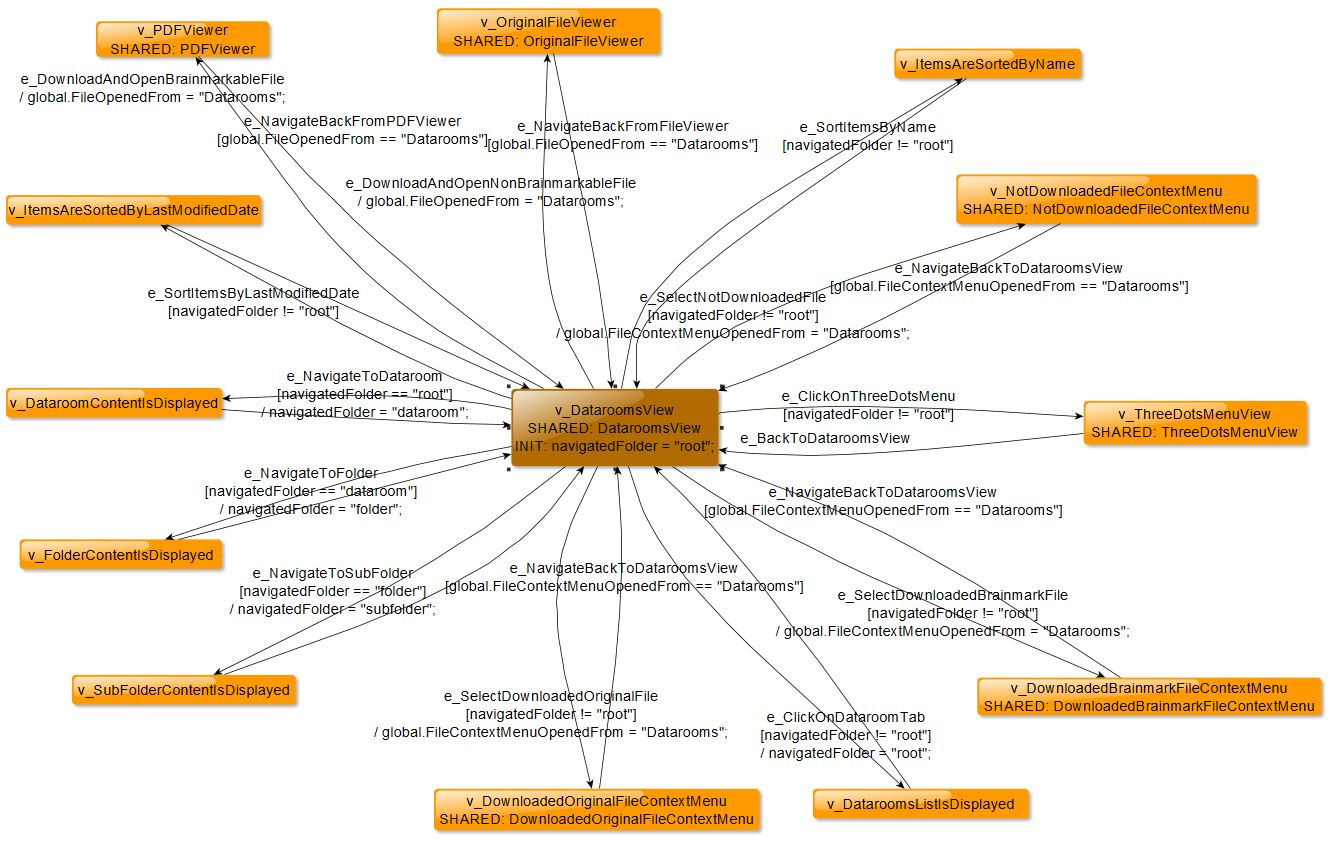
\includegraphics[width=1\textwidth]{figures/Datarooms_model_screenshot}
					\caption{\label{Fig:Datarooms_Model_Screenshot} Model for Datarooms Tab}
\end{figure}

\subsubsection{Modeling of Context Menus}
\par
The datarooms tab has four different context menus. The context menu for the current dataroom or the folder provides the option to create a new folder, upload or download a file and delete all locally saved folders under the current folder or the dataroom. The model for the context menu has 11 states and 18 transitions which can be observed in the figure below. The context menu for the original files that have been downloaded provides options for setting or unsetting the file as a favorite, viewing all the versions of the file, showing votes to which the selected file is attached to, deleting the file from the device and sending the file securely to an internal or external email address. This context menu is modeled with 10 states and 21 transitions. The context menu for the protected PDF files that have been downloaded provides options similar to the downloaded original file's context menu and additionally the user can share the review of the file with users that have been invited to the dataroom where the file is located. This context menu is modeled with 11 states and 24 transitions. The context menu for the files that are not downloaded provides options similar to the one for downloaded files, but instead of the option for deleting the file locally, it gives the option to download the original file. This context menu is modeled with 9 states and 18 transitions.

\begin{figure} [htbp!]
	\centering
					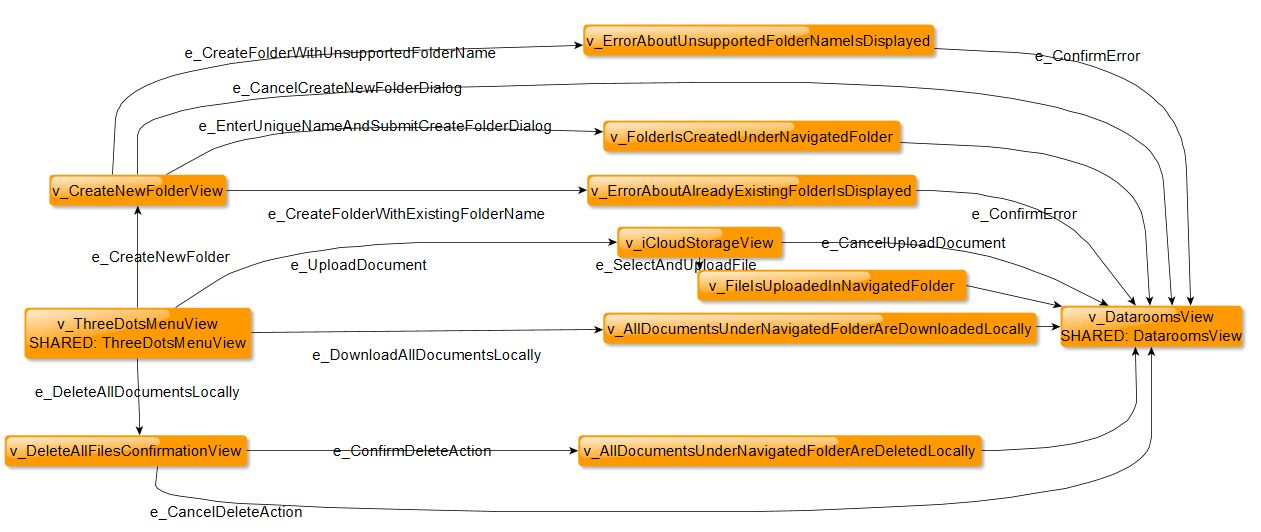
\includegraphics[width=1\textwidth]{figures/Context_Menu_model_screenshot}
					\caption{\label{Fig:Context_Menu_model_screenshot} Model for Dataroom Context Menu}
\end{figure}

\subsubsection{Modeling of the PDF Viewer}
\par
The PDF Viewer is one of the most important features of the \acrshort{bsc}. It allows the user to open and read through the protected PDF files that are generated, it also allows changing its views to fit to the page, fit to the width or fit to the height of the document as well as changing the layout of the document as single page continuous or single page. The user can perform a search using different keywords and navigate to the searched items found in the documents using the search module. The PDF document can be exported for printing directly from the PDF viewer or it can be exported to other applications on the device such as the Notes application. The user is able to bookmark the pages within the document, and access them conveniently through the thumbnails view. The different reviews can be accessed directly using the PDF viewer's Reviews view and they can be directly shared to the internal dataroom users. All of this functionality is embedded within the PDF Viewer's Operations model. It contains 31 states and 58 transitions.

\par
The next huge set of functionalities comes with the possible annotations available within the PDF viewer. There are four types of annotations: fineliner, pen, text and sticky notes. Other than these the eraser is also provided for deleting the fineliner and the pen annotations either completely or partially. The user can create, edit or delete an already created type of annotation. The editing of the fineliner and pen annotations includes changing the color, the thickness and the opacity of the annotation. The user can edit the size and the color of the text annotation as well as the content of the text itself. The sticky note annotations can be altered by changing the text. The annotation related behaviour of the PDF viewer is Modeled as the PDF Viewer Annotations model and consists of 26 states and 49 transitions.

\par
Unfortunately, due to the huge size of the models, none of them can be represented visually in this thesis since the reader will not be able to read and understand all the labels of states and transitions.

\subsection{Modeling of the Settings Tab}
\par
Settings tab allows the user to configure the internal settings of the application according to their needs. 
\par
Through the application view settings the user can set the default starting tab of application after entering the access code, they can hide and show the events and votes tab and if auto-indexing is enabled and configured within the dataroom the user can show and hide these indexes. 
\par
The access code settings allow the user to change the access code.
\par
The security settings allow the user to change the password for already connected accounts, reset the secondary authentication, log out of all the configured dataroom server accounts, set the period for the auto lock functionality, allow or restrict a user from copying texts through \acrshort{bsc} and pasting them in some other applications. Also the user can deny or allow the device to include data from \acrshort{bsc} into the iOS backup. 
\par
The download settings can be used in case the user wants to activate, deactivate or set default download period of the items in synchronized datarooms. They can observe the ongoing downloads in the download settings as well. Also, the user can restrict the app from using mobile data for downloads, or in turn allow it. 
\par
Through the deletion settings the user can delete all local content of the application, they can set the default time period after which local documents will be automatically deleted and can also reset the application completely which will delete all local content, will log out from all logged in accounts and will reset the defined access code.
\par
The servers and datarooms settings allow the user to add or remove dataroom servers, as well as synchronize or remove datarooms from added dataroom servers to which they have been invited.
\par
The Support view allows the user to access and read through data such as the user guide, setup guide as well as the legal and data protection notices. The user is also able to send log files or contact Brainloop's support via the dedicated tab and can access the customer service portal.
\par
The settings functionality is split up into 11 models. One main model is responsible for navigation between listed settings. It can be observed in the figure below. Each of the 7 settings of \acrshort{bsc} have a dedicated model. Additionally 3 models are created for the security, servers and datarooms settings as they were complex and required splitting.

\begin{figure} [htbp!]
	\centering
					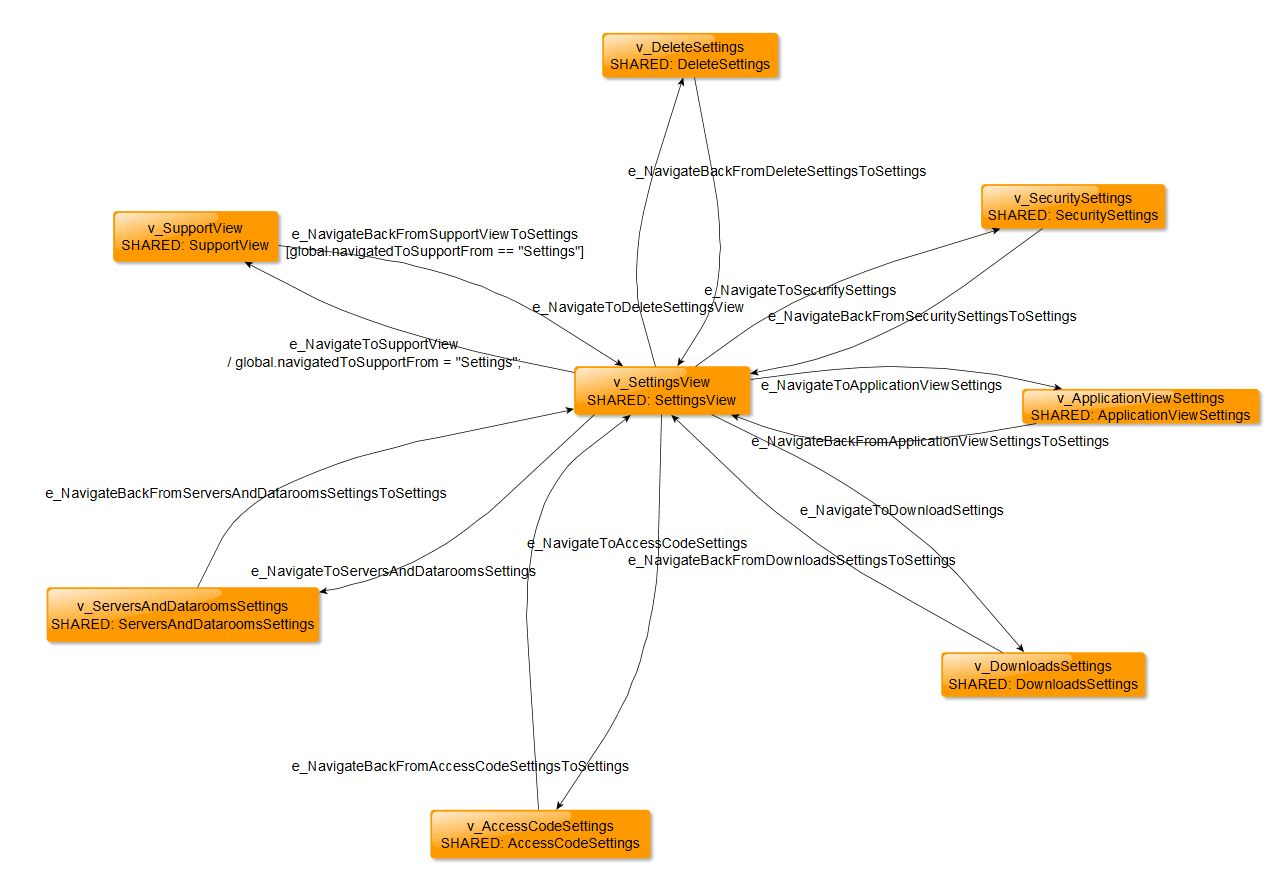
\includegraphics[width=1\textwidth]{figures/Settings_model_screenshot}
					\caption{\label{Fig:Settings_model_screenshot} Model for Settings Tab}
\end{figure}

\section{Layers}
\par
The generated models are structured in a layered manner. Accessing a specific functionality requires passing through all the layers between the base layer and the layer where the functionality is described. The ideal condition here would be if none of models depend on any model below the layer where it resides. But, unfortunately, in some cases this can not be achieved. For instance, the application view settings will define which tab the user will land on after entering the access code. The landing on a specific tab is decided within the enter access code model that resides in the base layer. Figure \ref{Fig:Layers} describes detailed structure of layers of our models.

\begin{figure} [htbp!]
	\centering
					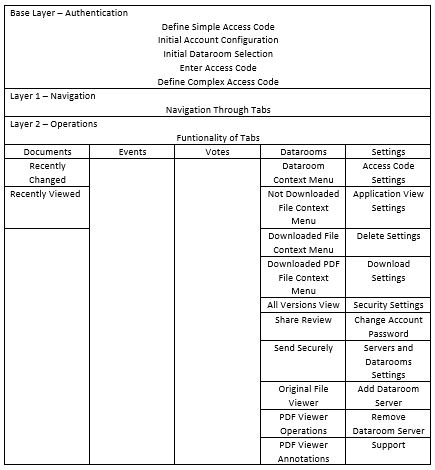
\includegraphics[width=0.8\textwidth]{figures/Layers}
					\caption{\label{Fig:Layers} Layered Structure of Models}
\end{figure}

\section{Modeling Overview}
\par
Overall, a total of 33 models were created, which consist of 312 states and 566 transitions describing the behavior of the \acrshort{bsc}. More detailed representation of the states and the transitions can be observed in the Table \ref{tab:Behavioral_models}.


\begin{table}[]
    \centering
    \begin{tabular}{|l|l|l|}
        \hline
        \textbf{Model Name} & \textbf{States} & \textbf{Transitions} \\
        \hline
        Datarooms & 13 & 25 \\
        \hline
        Dataroom Context Menu & 11 & 18 \\
        \hline
        Define Complex Access Code & 5 & 7 \\
        \hline
        Define Simple Access Code & 7 & 10 \\
        \hline
        Documents & 5 & 20 \\
        \hline
        Recently Changed & 7 & 10 \\
        \hline
        Recently Viewed & 7 & 10 \\
        \hline
        Enter Access Code & 8 & 11 \\
        \hline
        Events & 16 & 30 \\
        \hline
        All Version View & 3 & 4 \\
        \hline
        File Context Menu - Downloaded & 10 & 21 \\
        \hline
        File Context Menu - Not Downloaded & 9 & 18 \\
        \hline
        File Context Menu - Downloaded PDF & 11 & 24 \\
        \hline
        Share Review & 12 & 19 \\
        \hline
        Send Securely & 13 & 23 \\
        \hline
        Initial Account Configuration & 6 & 9 \\
        \hline
        Initial Dataroom Selection & 9 & 13 \\
        \hline
        Navigation Through Tabs & 6 & 25 \\
        \hline
        Original File Viewer & 4 & 6 \\
        \hline
        PDF Viewer Operations & 31 & 58 \\
        \hline
        PDF Viewer Annotations & 26 & 49 \\
        \hline
        Settings & 8 & 14 \\
        \hline
        Access Code Settings & 2 & 5 \\
        \hline
        Application View Settings & 9 & 16 \\
        \hline
        Delete Settings & 4 & 5 \\
        \hline
        Download Settings & 9 & 16 \\
        \hline
        Security Settings & 10 & 18 \\
        \hline
        Change Account Password & 5 & 6 \\
        \hline
        Servers and Datarooms Settings & 14 & 22 \\
        \hline
        Add Dataroom Server & 5 & 6 \\
        \hline
        Remove Dataroom Server & 4 & 4 \\
        \hline
        Support & 8 & 14 \\
        \hline
        Votes & 15 & 30 \\
        \hline
        \textbf{Total} & \textbf{312} & \textbf{566} \\
        \hline
    \end{tabular}
    \caption{Behavioral Models of \acrshort{bsc}}
    \label{tab:Behavioral_models}
\end{table}














